\section{Motivating Example}
In this section, we first give a brief description of update language twinning. Then, we
will give some examples to show why twinning cannot preserve the type correctness while
updating programs. Finally,
we will informally present an overview of our work.
\label{example}
\begin{figure}
    \centering
    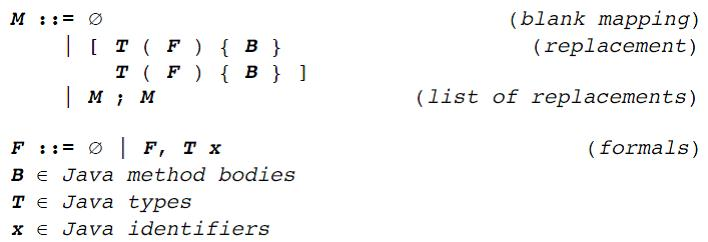
\includegraphics[width=8.5cm]{one}
    \caption{Syntax of twinning}
    \label{fig-syntax}
\end{figure}

\begin{figure}
    \centering
    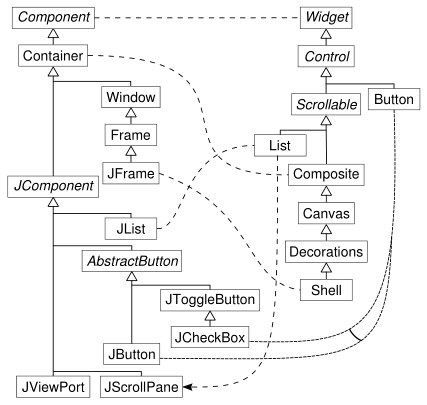
\includegraphics[width=7.5cm]{two}
        \caption{One option for Swing and SWT type mapping}~\cite{icsm2010}
    \label{fig-swingtoswt}
\end{figure}
Twinning is a rule-based language which describes the program modification to adapt to 
a new API. 
Twinning is very simple and easy to learn, as well as useful for its
powerful expressive ability.
Figure \ref{fig-syntax} shows the syntax of twinning which is restricted to the specification of single 
replacements. The main body of twinning is \textit{mapping}. A mapping M is a list of replacements, and
a replacement:

\begin{align*}
    [ &\quad T_{1} \quad ( \quad F_{1} \quad ) \quad \{ \quad B_{1} \quad \} \\
      &\quad T_{2} \quad ( \quad F_{2} \quad ) \quad \{ \quad B_{2} \quad \} \quad]
\end{align*}

\noindent consists of two nameless procedures, means replace $B_{1}$ with 
$B_{2}$. 
$T_{1}$ shows the type of $B_{1}$, and type list $F_{1}$ illustrates the
type of all the variables in body $B_{1}$. Similar with $B_{2}$. 
Type list of $F_{1}$ is point-wise related to the type list of
$F_{2}$. When a replacement was applied in a Java program, $B_{1}$ will match a code block 
(usually is a expression), then replace the code block with $B_{2}$.
Next, we will illustrate how twinning try to preserve type correct.


%详细说明twinning的type checking
First, twinning computes the type-mapping between former API and new API
According to collect type pairs from rules:
\begin{align*}
    &TypeMapping(\phi) = \phi \\
    &TypeMapping([T_{r}\,(T_{1}\,x_{1},\cdots,T_{n}\,x_{n})\; \{\,B\,\} \\
    &\quad\quad\quad\quad\quad\quad\quad T'_{r}\,(T'_{1}\,y_{1},\cdots,T'_{n}\,y_{n})\; \{\,B'\,\}]) \\
    &\quad={(T_{r},T'_{r}),\,(T_{1},T'_{1})\,\cdots,(T_{n}, T'{n})}\\
    &TypeMapping(M;M')\\
    &\quad =TypeMapping(M)\cup TypeMapping(M')
\end{align*}

Twinning demands that the type mapping is a function: $\forall T_{i}$, $\exists$ 
only one $T'_{i}$, that $T_{i}$ map to $T'_{i}$. 
There is a type checking while rules are matching the Java programs.
While a rule is matching a expression,
the types of variable in expression should being matched with type list in a rule
and type of the expression should match return type of the rule. 

We can see that twinning restrict the type mapping as a function and add a type checking while do
the match.
All this seems work good to preserve the type correctness while updating a program, 
but is this really enough to
preserve the type correctness?
Consider the API alternative from Swing to SWT, the inheritance relationship of classes in these two APIs lists in 
Figure \ref{fig-swingtoswt}. In figure \ref{fig-swingtoswt}, all the
mapping of classes is function, so we can use twinning to write rules about updating these classes. 
Some of the rules as follow:

\begin{verbatim}
[ Container () { return new Container(); }
  Composite () { return new Composite(PAR, N); } ]

[ JList () { return new JList(); } 
  List () { return new List(); } ]

[ JFrame () { return new JFrame(); }
  Shell () { return new Shell(); } ]
\end{verbatim}

\noindent PAR and N are default values provided for constructor of class Composite.
It seems right while using these rules to update clients with API Swing, 
but consider following statement in a type-safety client program:

\begin{lstlisting}[language=Java]
Container x = new JList();
\end{lstlisting}

\noindent If we update this statement with rules above, it will introduce a type error 
in the updated client.
The updated client code will be:
\begin{lstlisting}[language=Java]
Composite x = new List(); 
\end{lstlisting}
JList is a subtype of Container, but List is not a subtype of Composite. The cast of type List
to type Composite is a wrong cast, so the rules above cannot preserve the type correctness.
In our work, these rules will be excluded. 

The above example shows that the constraints of twinning is not enough to preserve the type
correctness while updating programs. Another example is about using HashMap as an alternative
class of class Hashtable. Part of methods in class Hashtable and the related class of Hashtable
as follows:

\begin{lstlisting}[language=java]
class Hashtable {
    Enumeration elements() { }
    boolean contains(Object v) { }
    Enumeration keys() { }
    ...
}
class Enumeration {
    boolean hasMoreElements() { }
    Object nextElement() { }
    ...
}
\end{lstlisting}

In this API alternative,
Class Hashtable maps to HashMap, and class Enumeration maps to class Iterator. The methods mapping
to methods listing above in HashMap and Iterator are as follows:

\begin{lstlisting}[language=java]
class HashMap {
    Collection values() { }            
    boolean containsValue(Object v) { }
    Set keySet() { }
    ...
}
class Collection {
    Iterator iterator() { }
    ...
}
class Set { 
    Iterator iterator() { }
    ...
}
class Iterator {
    boolean hasNext() { }
    Object next() { }
    ...
}
\end{lstlisting}

We can use SWIN to describe the mapping rules of this API alternative, the mapping rules:

\begin{verbatim}
[ Hashtable () { return new Hashtable(); }
  HashMap () { return new HashMap(); } ]

[ Enumeration (Hashtable x) { return x.elements(); }
  Iterator (HashMap x) { return x.values().iterator(); } ]

[ boolean (Enumeration v) { return v.hasMoreElements(); }
  boolean (Iterator v) { return v.hasNext(); } ]

[ Object (Enumeration v) { return v.nextElement(); }
  Object (Iterator v) { return v.next(); } ]
\end{verbatim}

From these rules, we can see method \textit{elements} in class Hashtable
maps to two methods \textit{values} in class HashMap and \textit{iterator} in
class Collection. We also require the bodies of these rules can be type checked,
and the type mapping is a function as twinning. But our paper want to make sure
all the clients using Hashtable should be update type safely. These rules are
not enough for our goal, we should assure that all the methods and classes in
Hashtable have replacements, such as methods \textit{contains} and \textit{keys} in class
Hashtable. Adding this condition, we can assure the clients
can be safely updated.


From these examples, we can see that invalid or incomplete rules in twinning 
may introduce type-errors
while updating client programs. In our paper, we should exclude invalid rules, 
and assure the all the valid rules in SWIN can preserve the type
correctness while updating any type-safety programs. 
In our paper, we give a set of properties that a type safe rule
should satisfy with, and we call these properties are type safe properties 
(short for safe properties). There are mainly three properties that rules
should satisfy with. Next, we will informally and briefly explain these two cases. 

Consider a rule:
\begin{align*}
    [ \quad &T_{1} \quad ( \bar{F} \quad \bar{x} ) \quad \{ \quad B_{1} \quad \} \\
     &T_{2} \quad ( \bar{G} \quad \bar{y}) \quad \{ \quad B_{2} \quad \} \quad]
 \end{align*}
 In rules above, $\bar{F}\; \bar{x}$ is short for $F_{1}\;x_{1},F_{2}\;x_{2},\cdots,F_{n}\;x_{n}$,
 same as $\bar{G}\;\bar{y}$. 

 \begin{itemize}
     \item In rule checking, first, it require that all the variables in
 $B_{1}$ should be binded with $\bar{x}$, and all the $\bar{x}$ are appearance in $B_{1}$. Second, it 
 need to assure that $B_{1}$ is a single body, 
 it means there is no more than one method invoke in $B_{1}$.

    \item We also collect the type mapping as twinning, and these type mapping should be a 
        function. All the methods in rules should cover all the methods in class appeared in rules, and
        for the methods in rules should type-safety according the definition of APIs. For any method
        not in rules, there should be a method in mapped class with same name, and the type of
        parameters and return value should satisfy the type mapping.

    \item The last properties is about inheritance. For the inheritance of classes in former API, 
        these relationship cannot be removed in new API of between any two classes after updated, and
        the adding of relationship between classes is allowed.
\end{itemize}
